\subsection{Planet yield from an example Extended Mission (\rm{\nhemi}) }
\label{sec:results_from_nhemi_extended_mission}

\begin{figure*}[t]
	\centering
	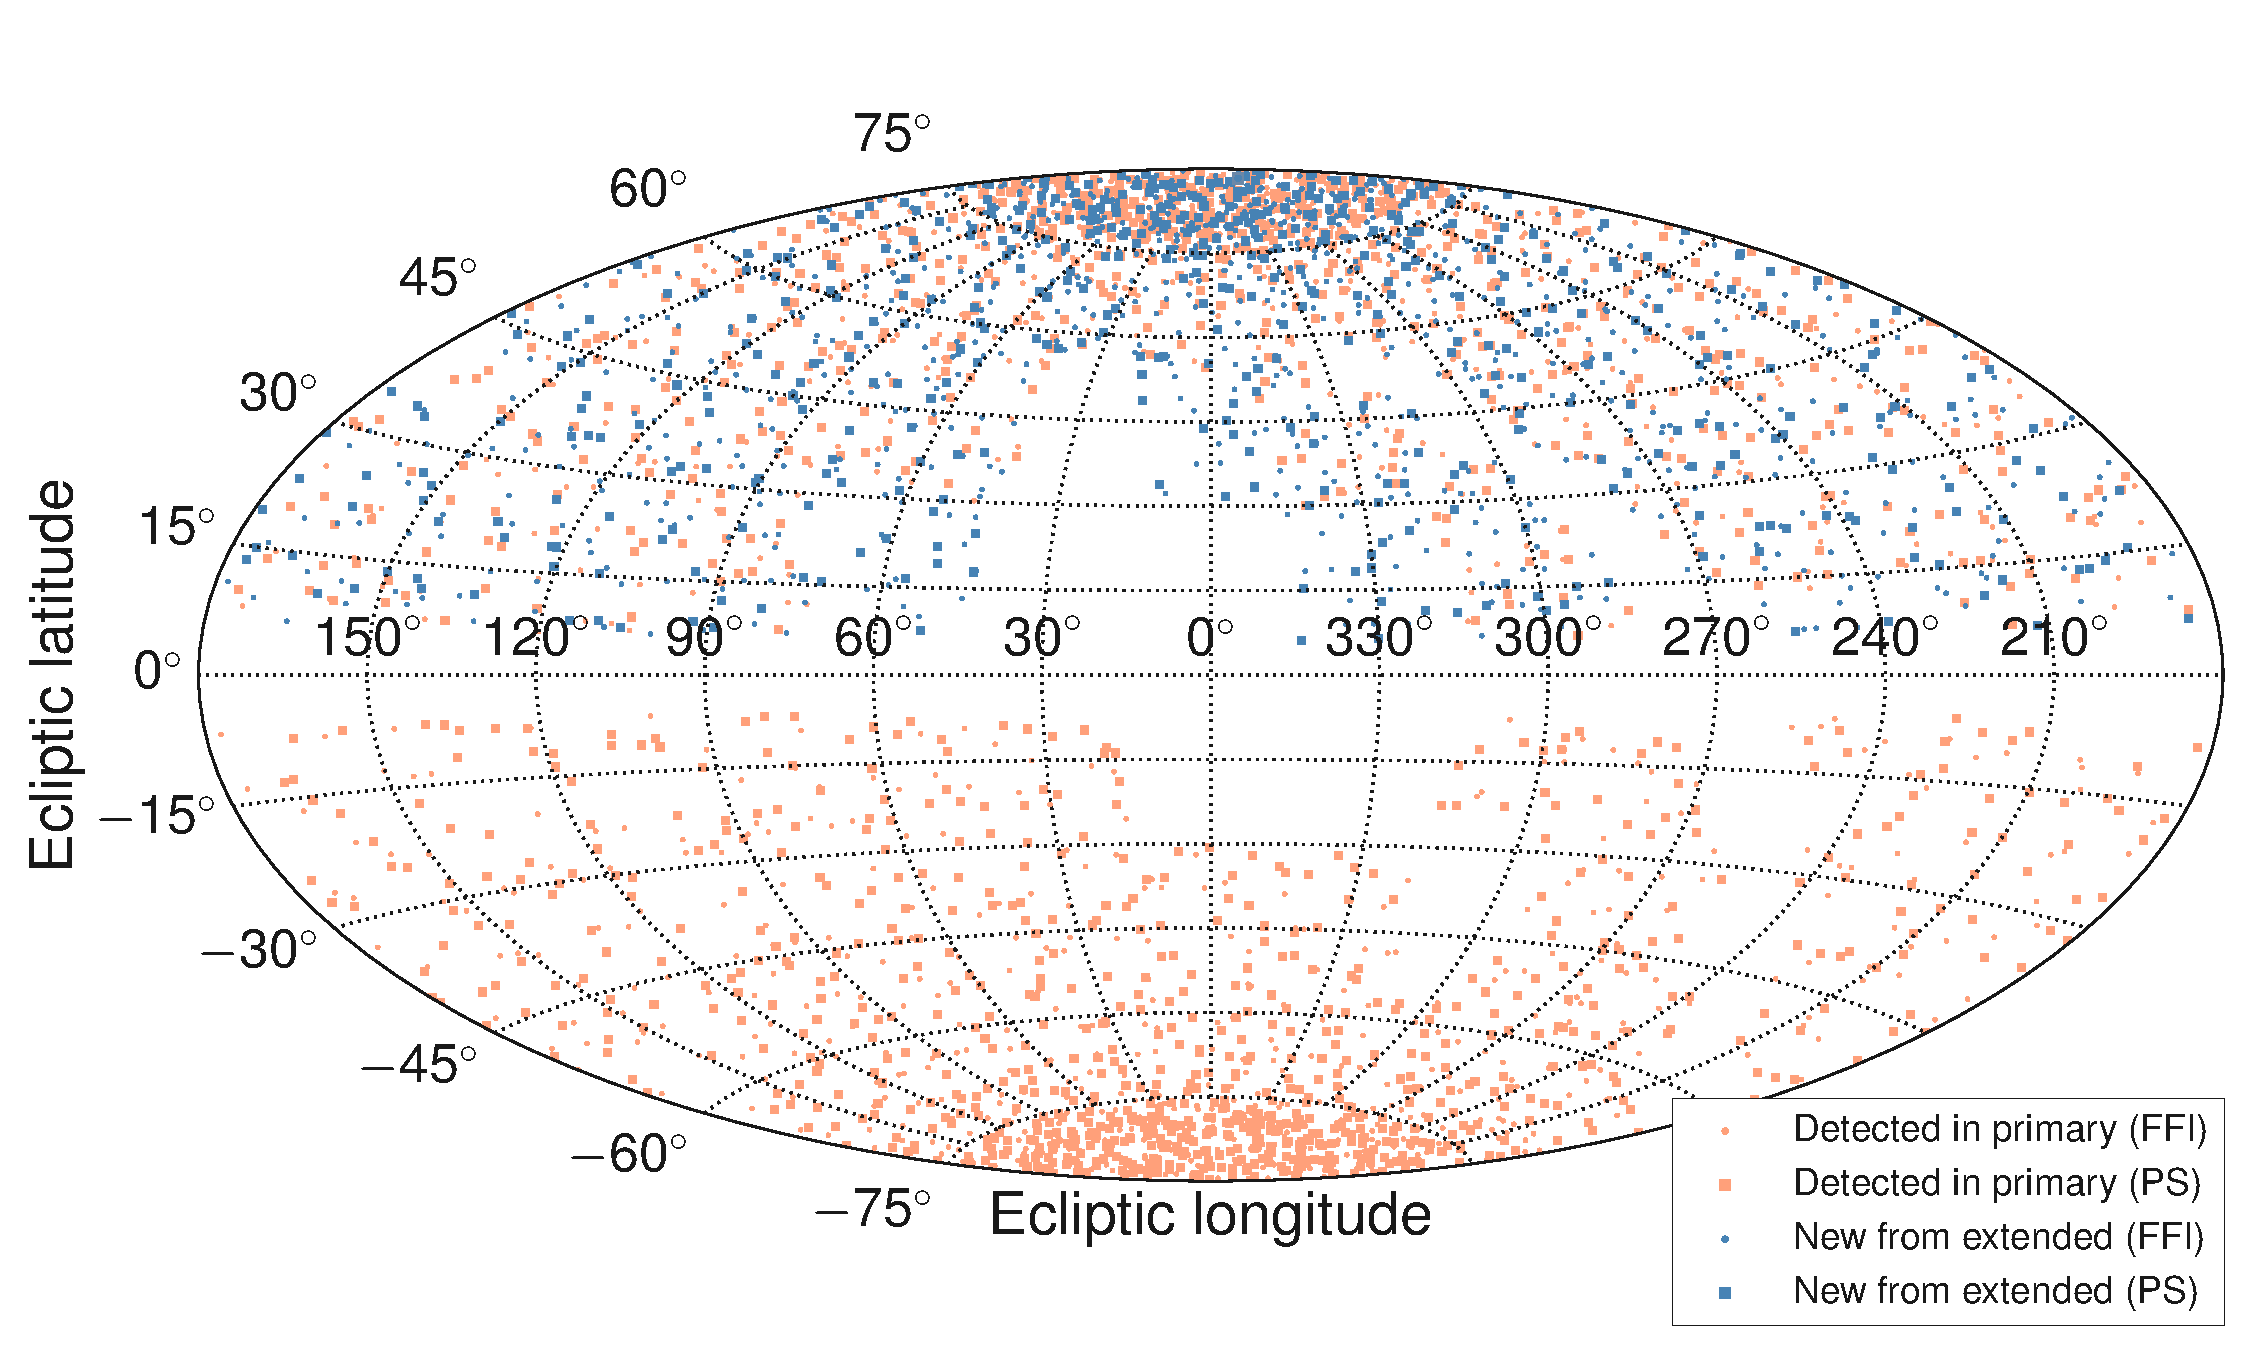
\includegraphics[]{figures/skymap_dropped_fields.pdf}
	\caption{Positions of $R_p<4R_\oplus$ planets detected in the \nhemi\ scenario. Squares (postage stamps) and dots (full frame images) are observed at 2 and 30 minute cadence respectively. Orange denotes detection over the first two years of observing (the Primary Mission), and blue denotes newly detected planets from the extra third year. The `gaps' in fields due to Earth and Moon crossings during the primary and Extended Missions are noted in Table~\protect\ref{tab:dropped_fields}. For instance, the field centered at $(\lambda=330^\circ,\beta=18^\circ)$ is observed in the extended but not the Primary Mission. }
	\label{fig:skymap_nhemi}
\end{figure*}
\begin{figure*}[t]
	\centering
	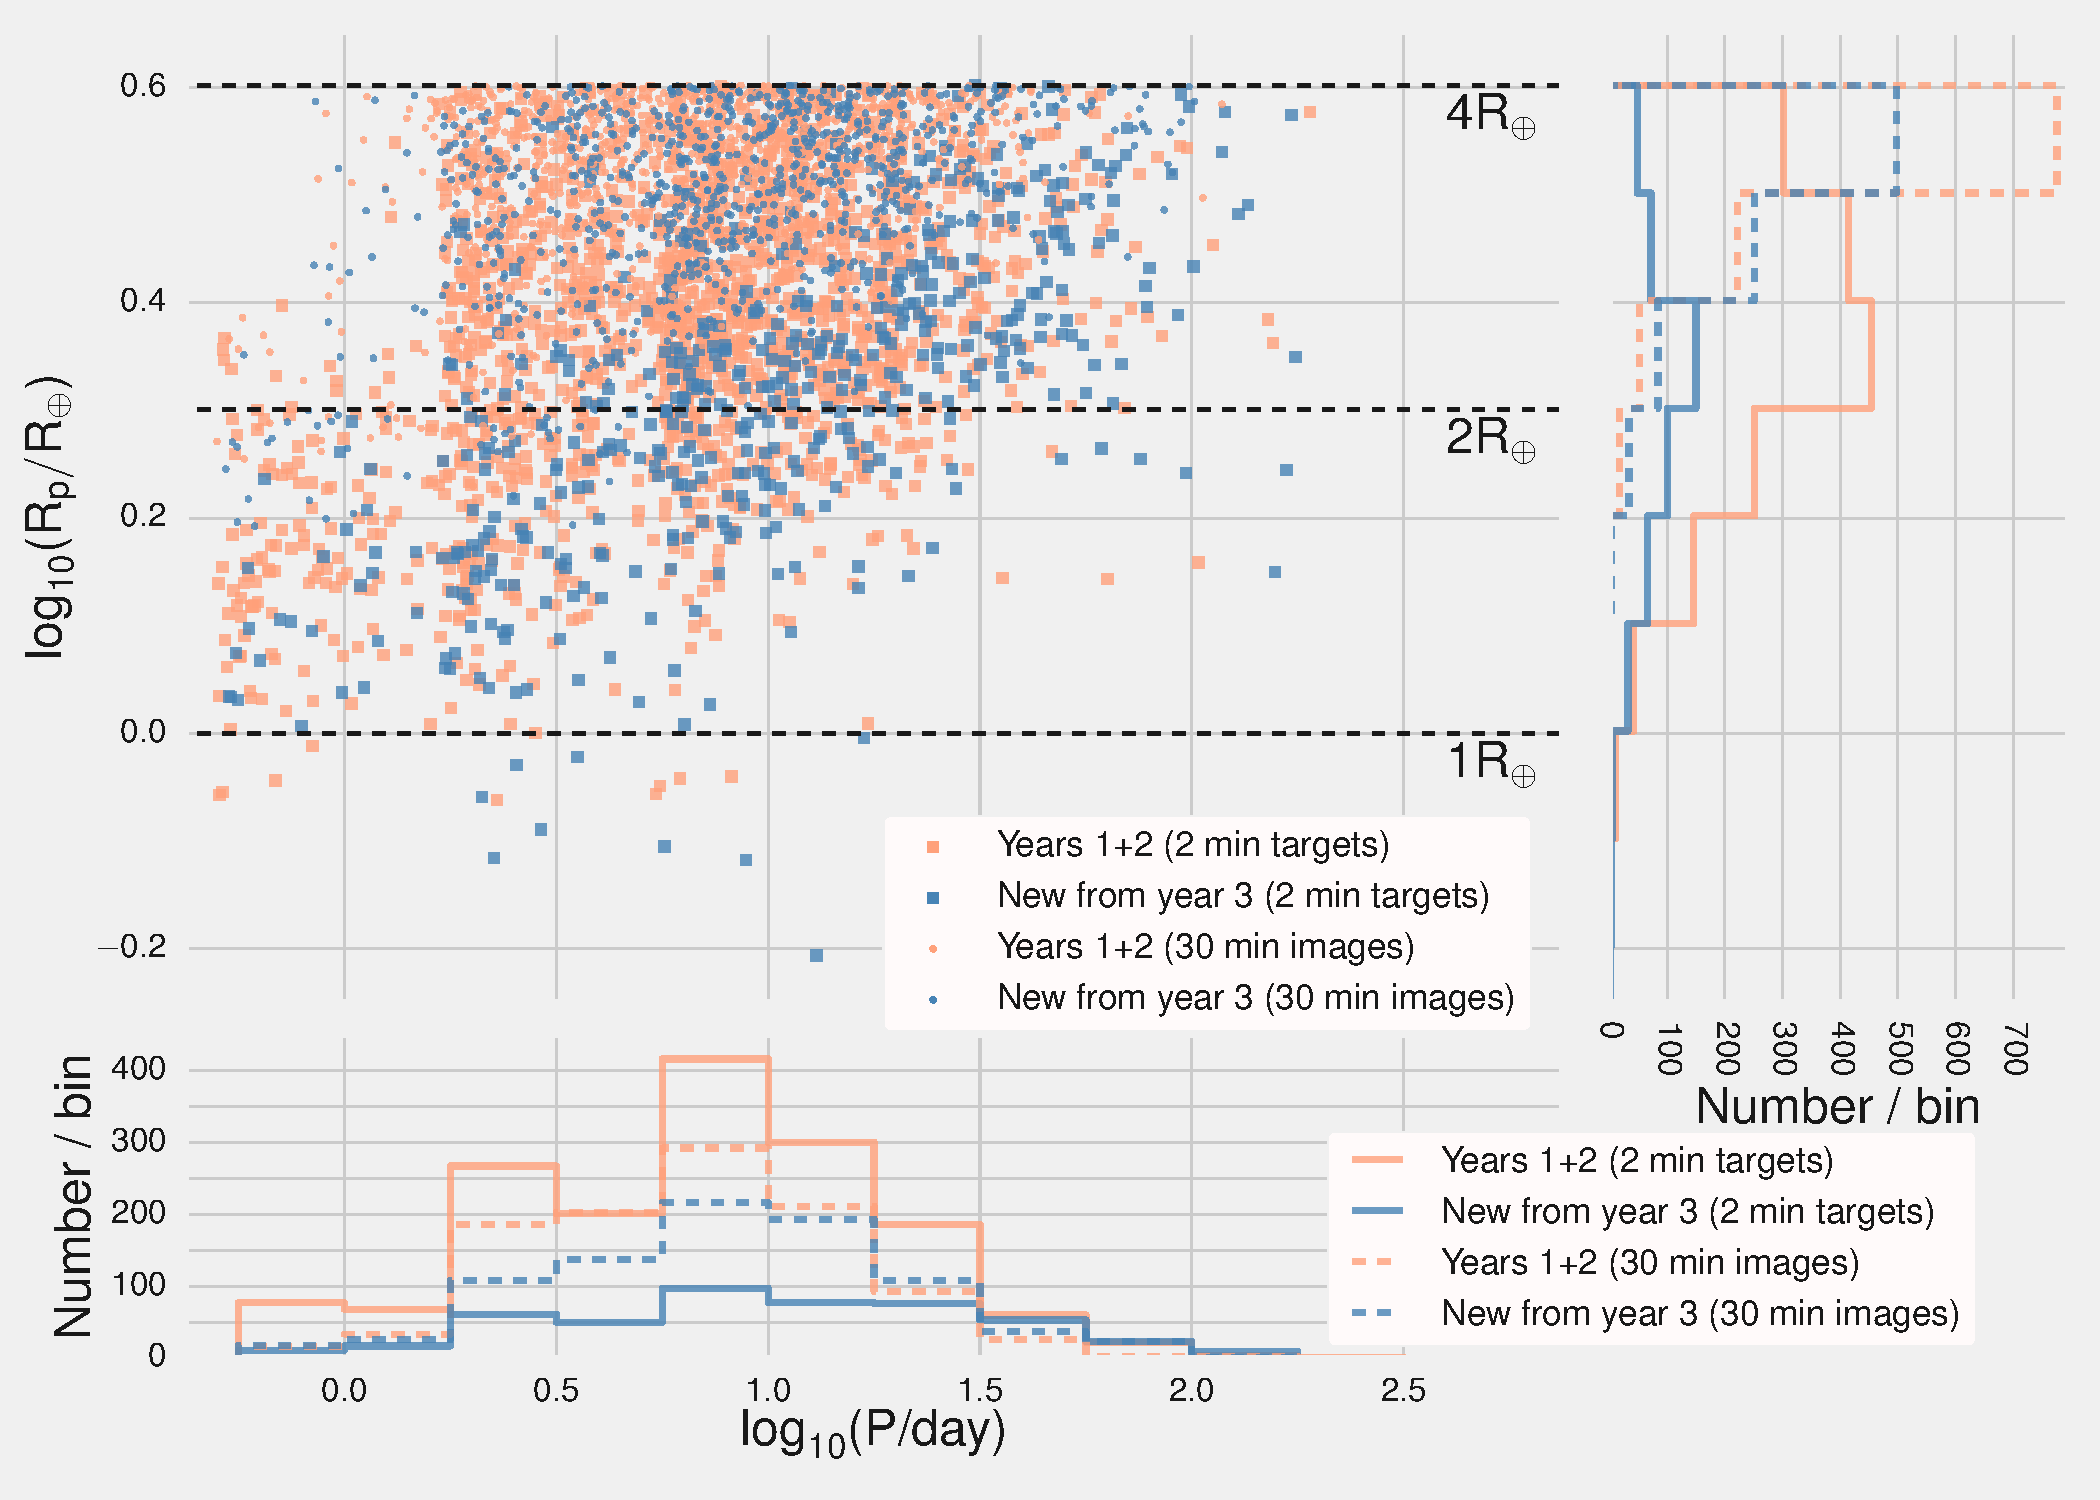
\includegraphics[]{figures/logR_vs_logP.pdf}
	\caption{Radius vs period of detected $R_p<4R_\oplus$ planets from one Monte Carlo realization of the \nhemi\ scenario.
	At a fixed period, Extended Missions help us detect smaller planets; at a fixed radius, they let us probe out to longer periods.
	The radius histogram, and the location of all dots (rather than squares) on the scatter plot show that almost all $R_p<2R_\oplus$ planets are detected in postage stamps, not full frame images (also shown in Fig.~\protect\ref{fig:primary_planet_yield}).}
	\label{fig:radius_vs_period_nhemi}
\end{figure*}
\begin{figure*}[t]
	\centering
	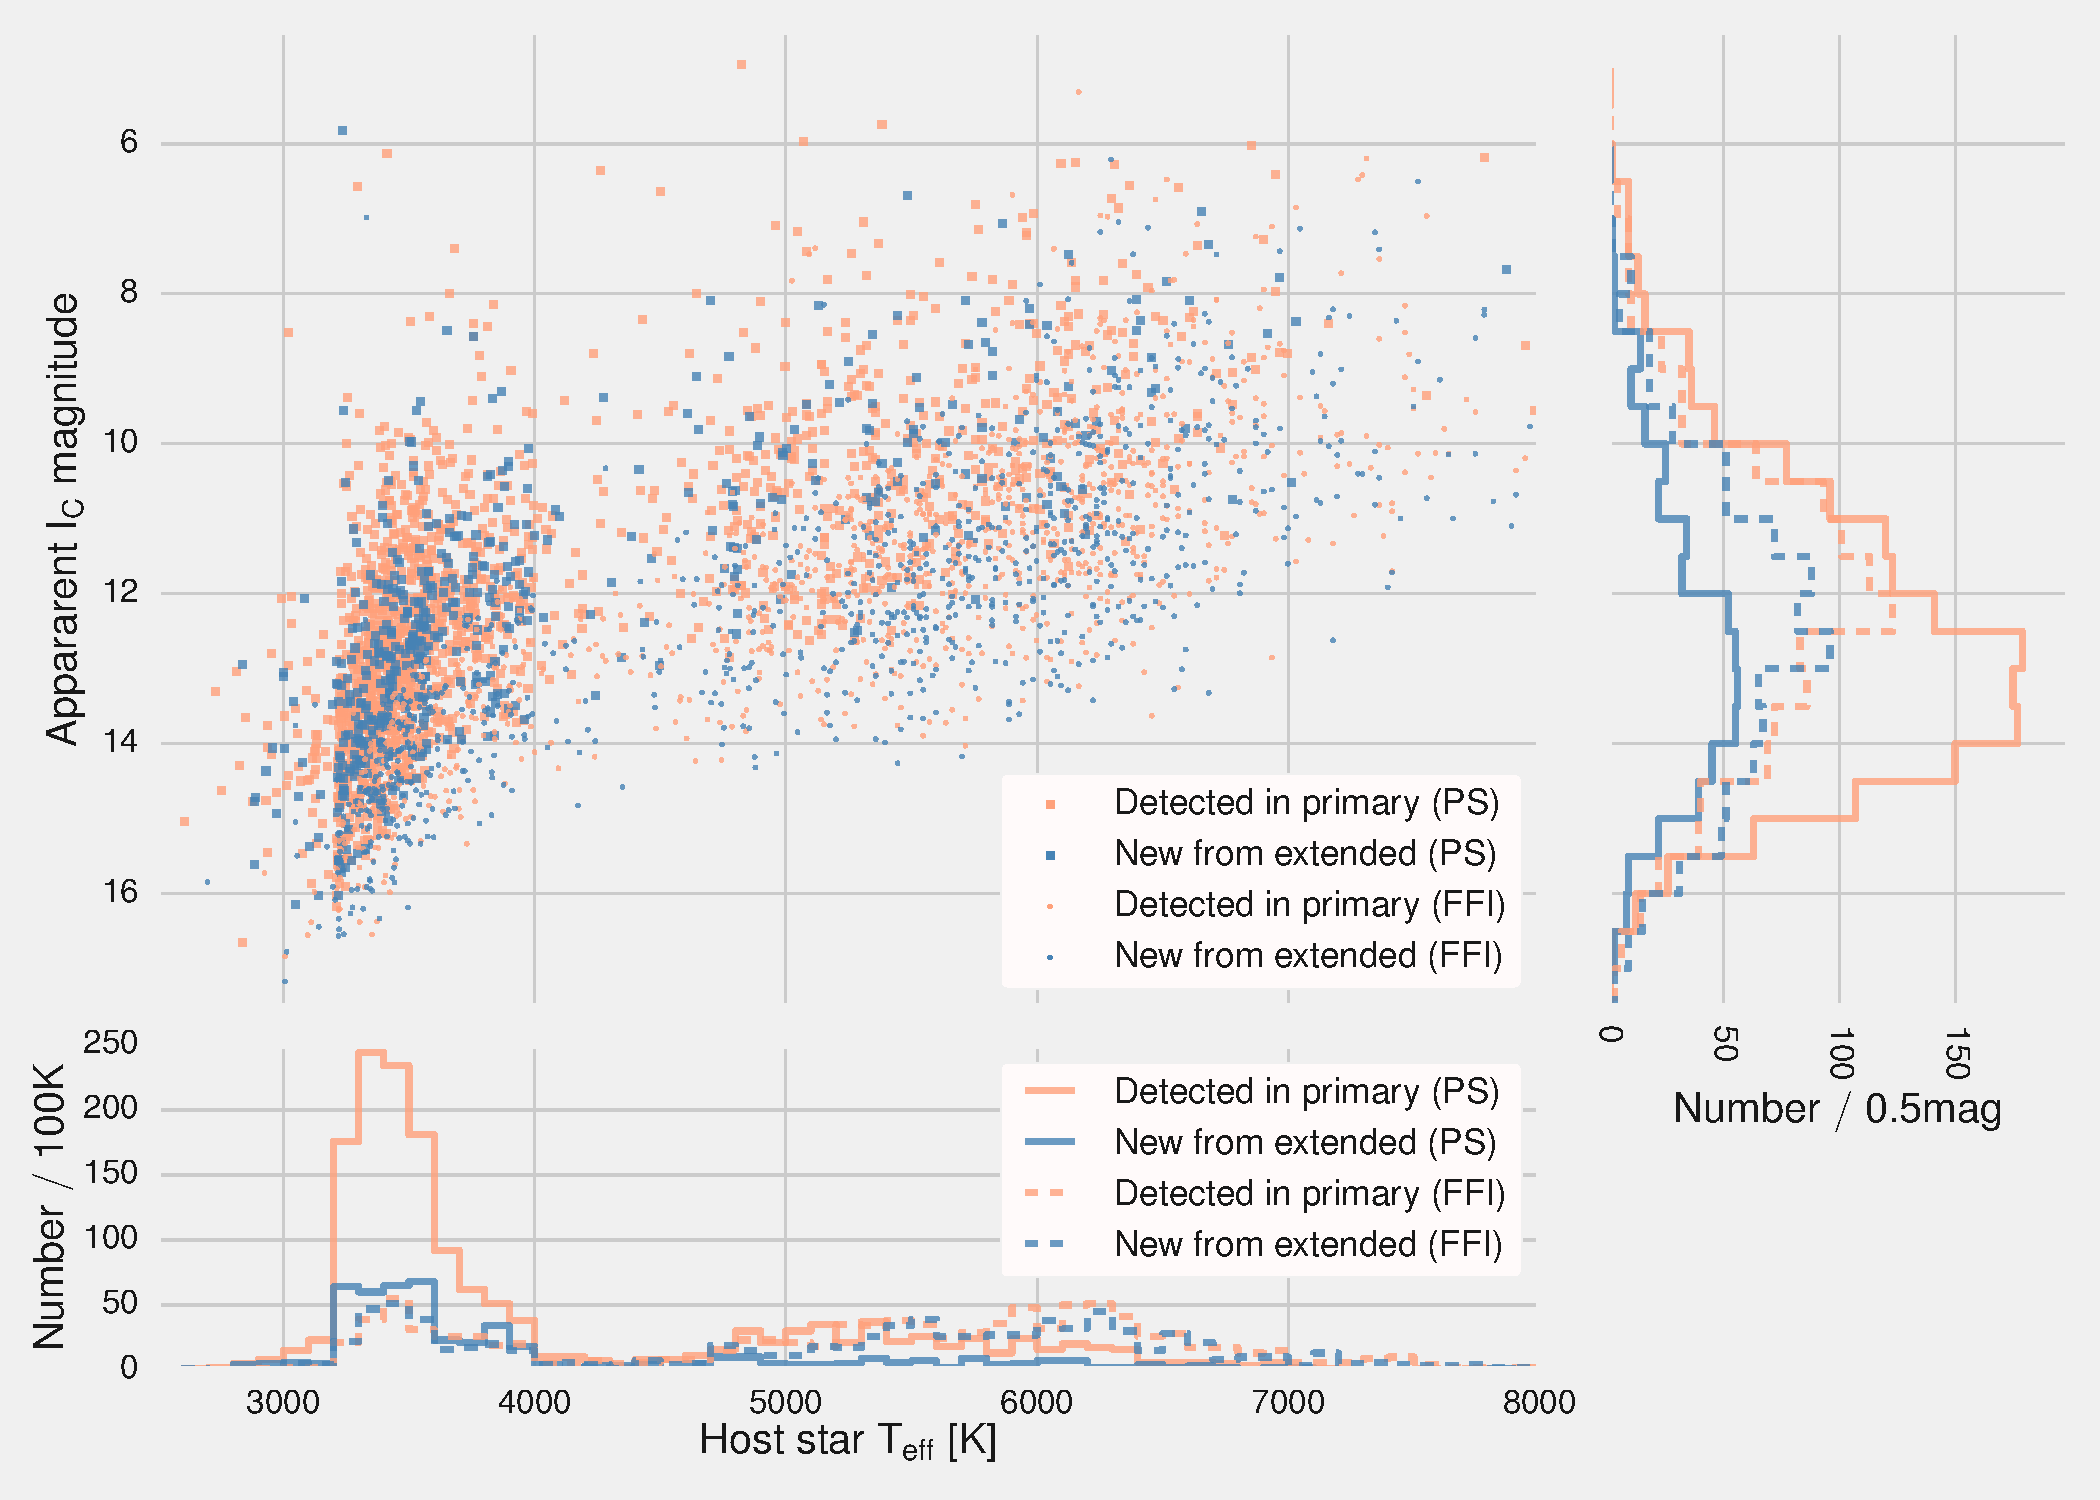
\includegraphics[]{figures/temp_imag_vs_teff_nhemi.pdf}
	\caption{Apparent Cousins I magnitude plotted against effective temperature for $R_p<4R_\oplus$ planets detected from one Monte Carlo realization of the \nhemi\ scenario. 
	Postage stamp (PS) detections are biased towards M dwarfs in part because of our selection procedure.
	For a given effective temperature, full frame images (FFIs) are taken of dimmer stars.}
	\label{fig:imag_vs_teff_nhemi}
\end{figure*}
	%all from 160729 runs. In this case for nhemi.

Before comparing our six selected Extended Mission scenarios simultaneously (Sec.~\ref{sec:results_from_all_extended_missions}), we describe the detected planet populations from a single realization of an Extended Mission.
As an example case, we choose the \nhemi\ scenario.

A sky map showing the positions of detected planets for this mission is drawn in Fig.~\ref{fig:skymap_nhemi}.
Commenting on this map, we note that:
\begin{itemize}
	\item Any planet detected in this scenario's Primary Mission is also detected in its Extended Mission.
	We consequently color the detected planets depending on if they are discovered in the Primary Mission, or whether they are detected only by virtue of the extra data collected in the Extended Mission.
	In our simulation, these extra observations will lead to new detections (a) because of an increased number of observed transits leading to a higher phase-folded SNR, which causes the transiting object's SNR to clear our threshold of 7.3, and/or (b) because raising the number of observed transits clears the minimum number of transits we require for detections ($N_\mathrm{tra} \geq 2$).
	\item The `dropped' fields described in Sec.~\ref{sec:earth_moon_crossings} owing to Earth/Moon crossings are visible for both the primary and Extended Missions in the $\lambda=(30^\circ, 0^\circ, 330^\circ, 300^\circ)$ fields.
\end{itemize}

In addition to examining the positions of the detected planets, we select and plot some of their key properties:
planet radius $R_p$, orbital period $P$, apparent magnitude $I_c$, and effective temperature $T_\mathrm{eff}$.
See Figs.~\ref{fig:radius_vs_period_nhemi} and~\ref{fig:imag_vs_teff_nhemi}.
Both of these figures are visualizations from a single Monte Carlo realization of the \nhemi\ scenario, and only show planets with $R_p < 4R_\oplus$.
These plots clarify a few points:
\begin{itemize}
	\item At a fixed period, Extended Missions help us detect smaller planets; at a fixed radius, they let us probe out to longer periods. This is one of the major reasons to extend \tesss observations.
	\item Almost all $R_p<2R_\oplus$ planets are detected in postage stamps, not full frame images. This is an indication that the top $2\times10^5$ \texttt{Merit} stars are a sufficient sample to detect most of the $R_p<2R_\oplus$ planets that \tess can detect.
	\item Postage stamp detections are biased towards M dwarfs. Per Fig.~\ref{fig:fig17_replica}, this is largely because our selection procedure chooses many M dwarfs.
	\item For a given effective temperature, full frame images detect planets about dimmer stars. Projecting the FFI detections onto apparent $I_c$ magnitude (Fig.~\ref{fig:imag_vs_teff_nhemi}, right panel), the median brightness of stars with planets detected from FFIs is actually greater than the median brightness of planets detected from PSs. This is because these detections are about stars with radii that, on average, are greater than those from postage-stamp detections.
	%\item The large number of full frame image detections between $5000\mathrm{K} < T_\mathrm{eff} < 7000\mathrm{K}$ suggest that our proposed selection procedure (Sec.~\protect\ref{sec:selection_criteria}) may not be optimal, and that a robust approach towards target prioritization, for instance using expected planet occurrence rates as a function of stellar type in a Bayesian approach, could maximize \tesss expected yield. 
\end{itemize}

There are a few other statistics that interesting for purposes of characterizing the value of this Extended Mission -- how many new planets do we detect? How many are at long orbital periods? How many are in habitable zones? We respond to these questions in Sec.~\ref{sec:results_from_all_extended_missions}, in particular showing our detected planet yields in Fig.~\ref{fig:yield_results}.
